\chapter{Navigatie brainstorm}
    \label{navigationappendix}
\textit{28 oktober 2009} Door middel van een brainstorm over de navigatie van Wakoopa is er een sitemap opgesteld. De brainstorm is uitgevoerd door het Team van Wakoopa (Wouter, Robert, Menno, Mark en Marten), wat betekent dat er voorkennis aanwezig was. Dit is deels tegengegaan doordat er twee personen bij waren die minder bekend waren met de huidige navigatie, Mark en Marten. Er is uitgegaan van een ingelogde status, een status waarbij de gebruiker toegang heeft tot zijn eigen gegevens. Statische pagina's zoals Privacy, About en FAQ zijn voor deze brainstorm buiten beschouwing gelaten, omdat ze niet actief deel hebben in gebruik van de website.

Van tevoren waren alle bestaande pagina's op post-its geschreven, en deze zijn verdeeld over de aanwezigen met de opdracht om deze gezamelijk op een A1 vel te plakken, waarbij gelijk pagina's geclusterd werden en de hi\"erarchie aangegeven werd door post-its onder elkaar te plakken. Hier werd expliciet gevraagd niet aan de huidige navigatie vast te houden, maar het zo neer te leggen dat het voor de personen zo logisch mogelijk was. Bijgevoegd waren pennen, waarmee de deelnemers toevoegingen of verduidelijkingen op of om de post-its konden schrijven.

\section*{Uitkomst}
De website werd ingedeeld in zeven hoofdsecties: Home, dashboard, application, people, teams, categories en developers. Dit is iets anders dan de huidige site, die Home/dashboard, Software, People en Search als hoofdsecties heeft. Het downloaden van de tracker staat momenteel onder het dashboard, maar werd liever direct onder Home gezien, met de beredenatie dat iedereen in principe de tracker mag downloaden. Een ander tweedeling is die van informatie over een gebruiker. Een deel daarvan hoort onder het dashboard (jouw persoonlijke accountpagina) en het ander onder You, je publieke profiel. Uit de workshop bleek dat een aantal van deze dingen niet op de goede plek stonden en beter zouden kloppen wanneer ze onder het persoonlijke dan wel publieke deel van Wakoopa zouden staan.
\section*{Vergelijking met \citeauthor{Hoekman2008}}
Kijkend naar de verbeteringen zoals voorgesteld door \citeauthor{Hoekman2008} (zie figuur \ref{miskeetonav2}) kun je zien dat de uitkomst van de workshop tussen de huidige site en de verbeteringen van \citeauthor{Hoekman2008} in zit. Hoewel de benaming en de pagina's hetzelfde blijven als op de huidige site, met slechts hier en daar een bijgeschreven verbetering, neigt de verdeling van de pagina's meer naar de indeling van \citeauthor{Hoekman2008}. Waar de verbeterde versie van \citeauthor{Hoekman2008} een compleet nieuwe indeling is, kwam er uit de workshop een gefinetunede versie van de huidige navigatie.

      \begin{figure}
      \begin{center}
      \caption{Huidige navigatie}
        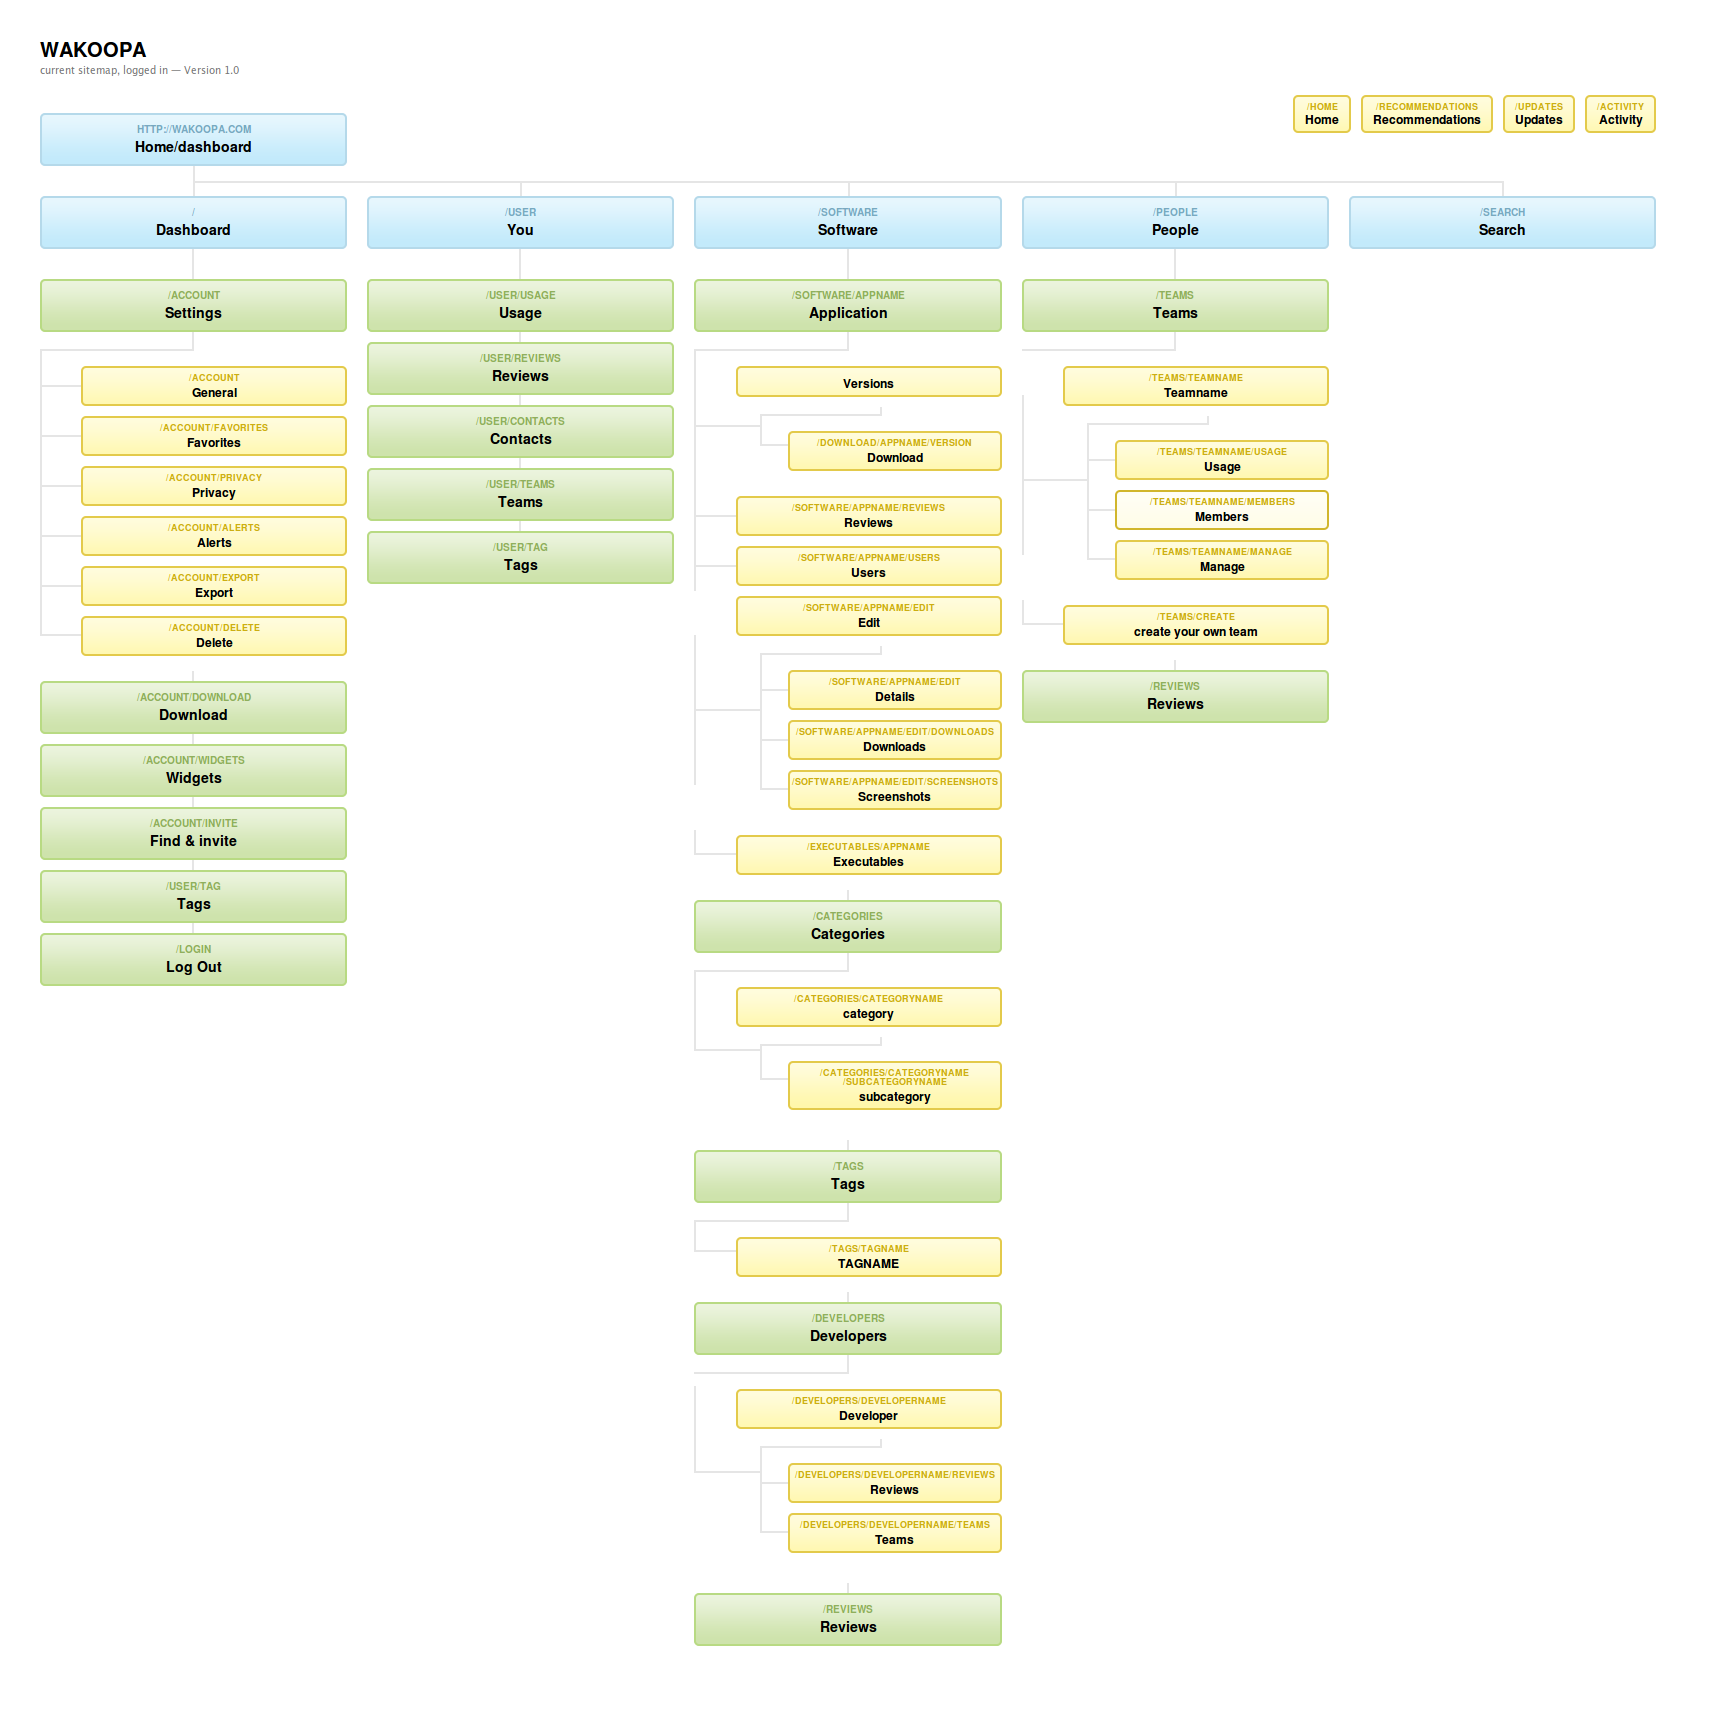
\includegraphics[width=\textwidth]{../images/currentnav}
      \end{center}
    \end{figure}

    \begin{figure}
      \begin{center}
      \caption{Verbeterde navigatie volgens \cite{Hoekman2008}}
        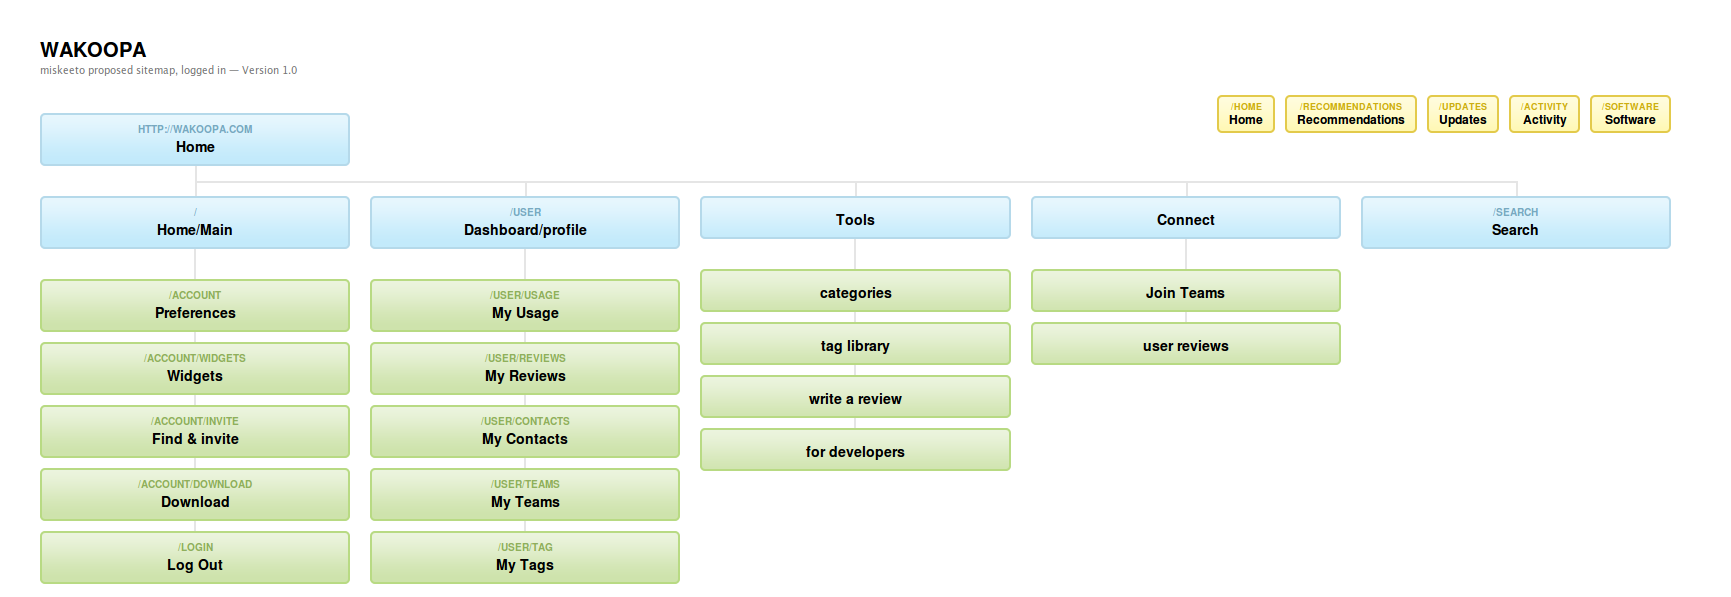
\includegraphics[width=\textwidth]{../images/miskeetonav}
      \label{miskeetonav2}
      \end{center}
    \end{figure}

      \begin{figure}
      \begin{center}
      \caption{Verbeterde navigatie volgens Navigatie workshop}
        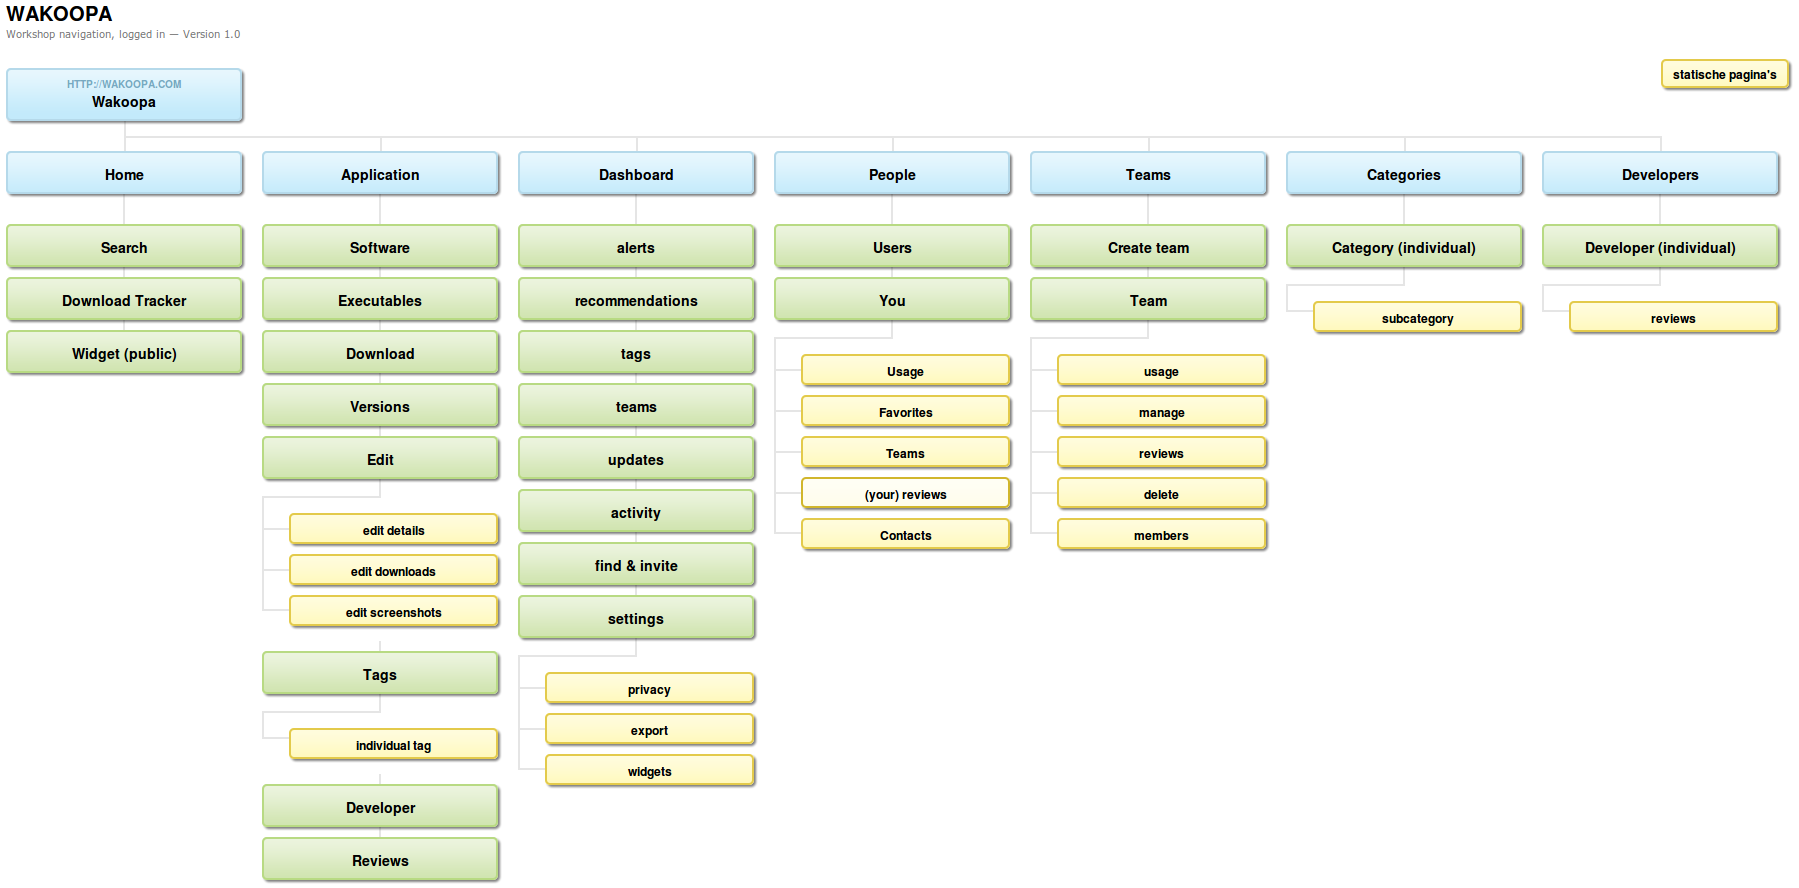
\includegraphics[width=\textwidth]{../images/workshopnav}
      \end{center}
    \end{figure}

    \begin{figure}
      \begin{center}
      \caption{Foto's van de workshop}
        \subfigure{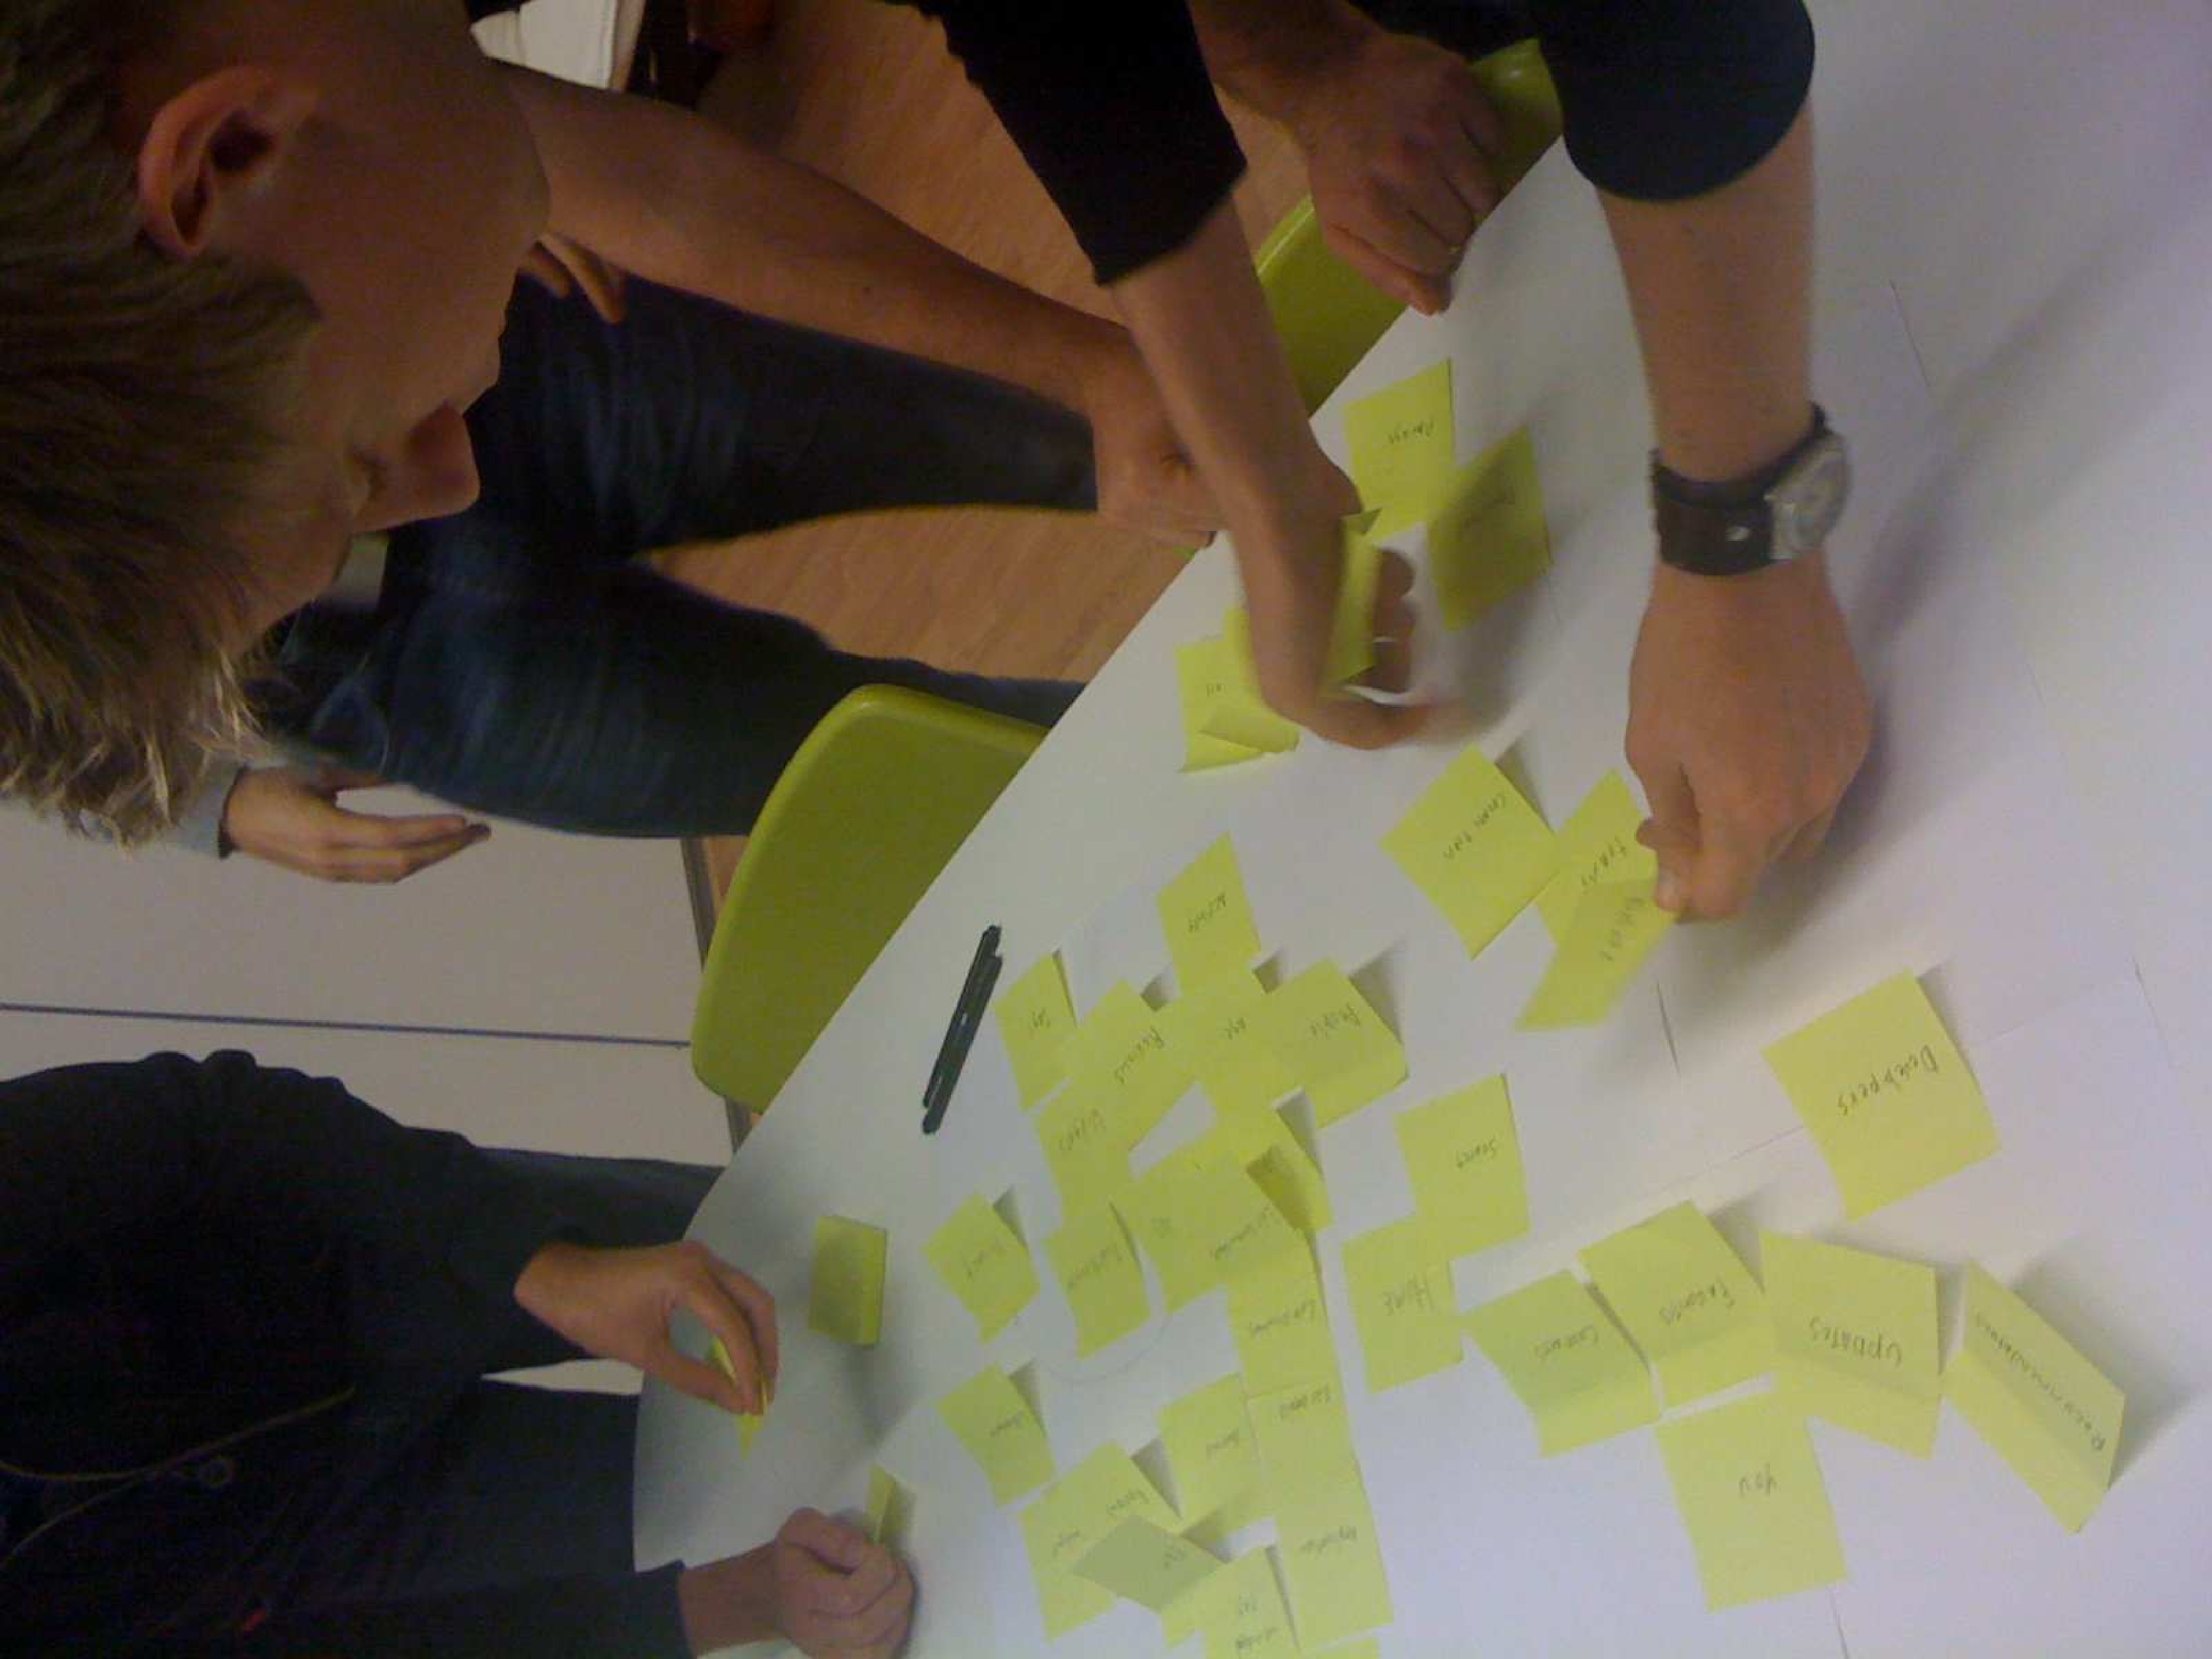
\includegraphics[height=6cm,angle=-90]{../images/navigatie-workshop/workshopimg1}}
        \subfigure{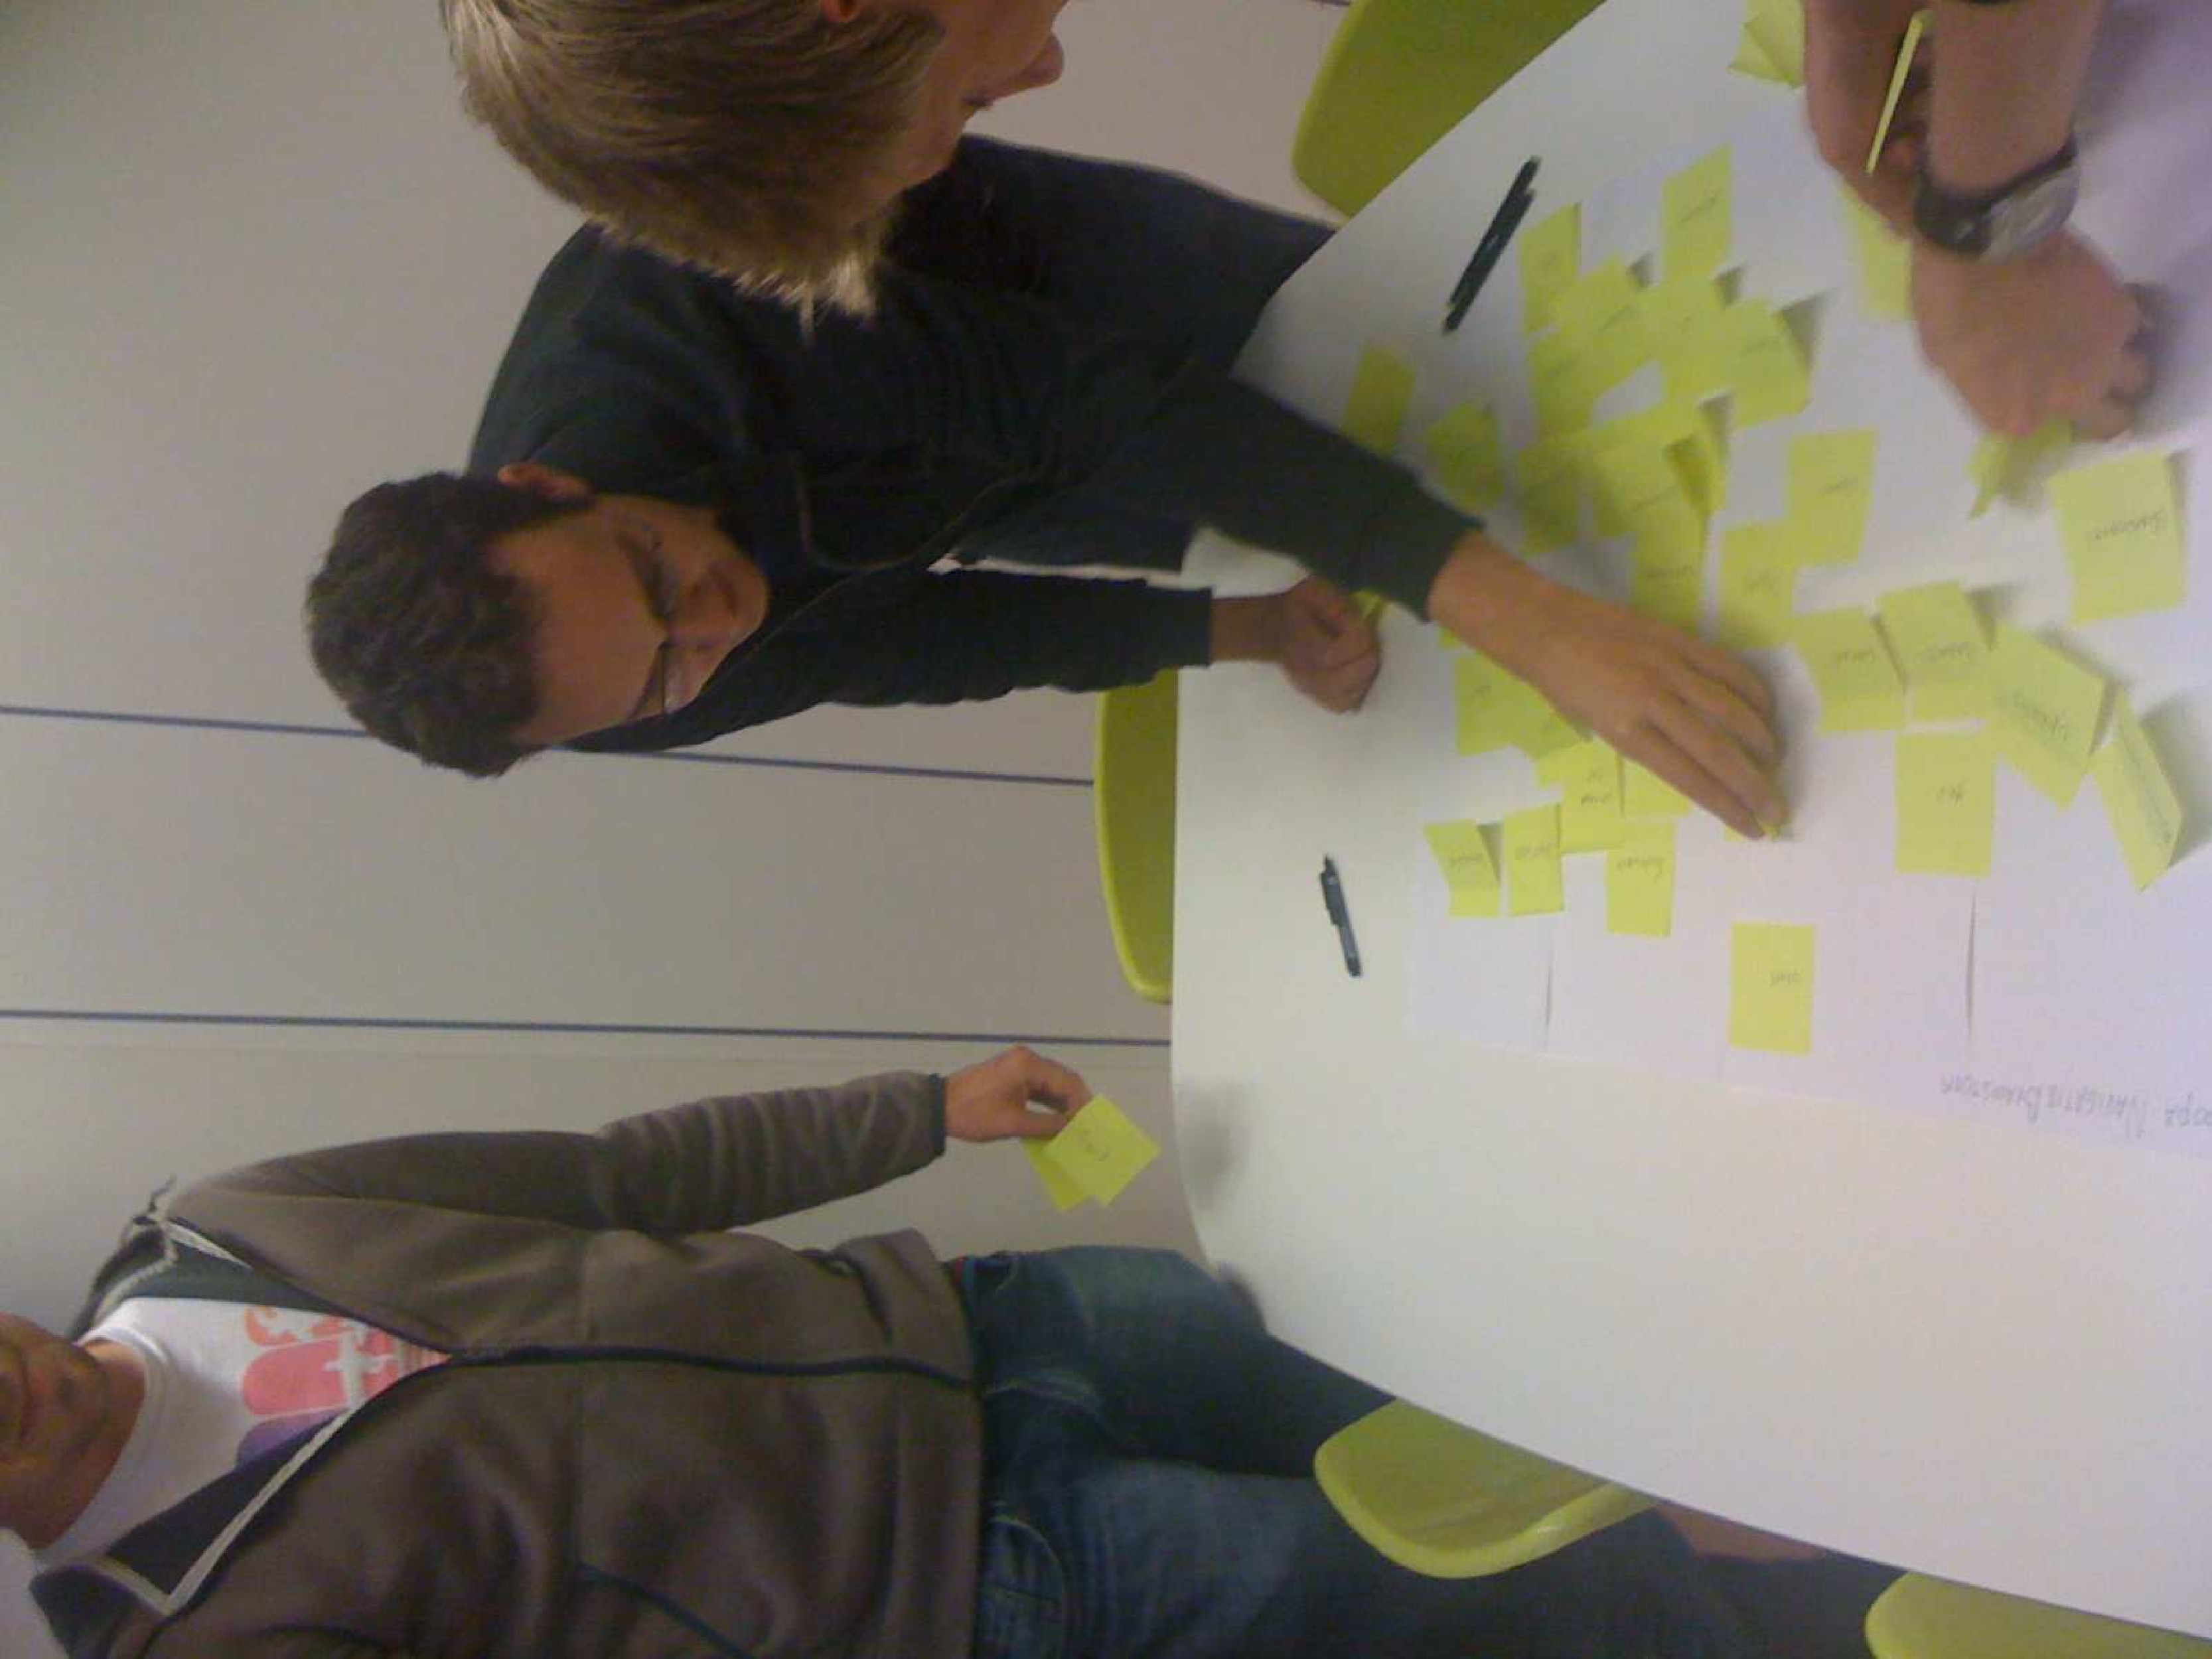
\includegraphics[height=6cm,angle=-90]{../images/navigatie-workshop/workshopimg3}}
        \subfigure{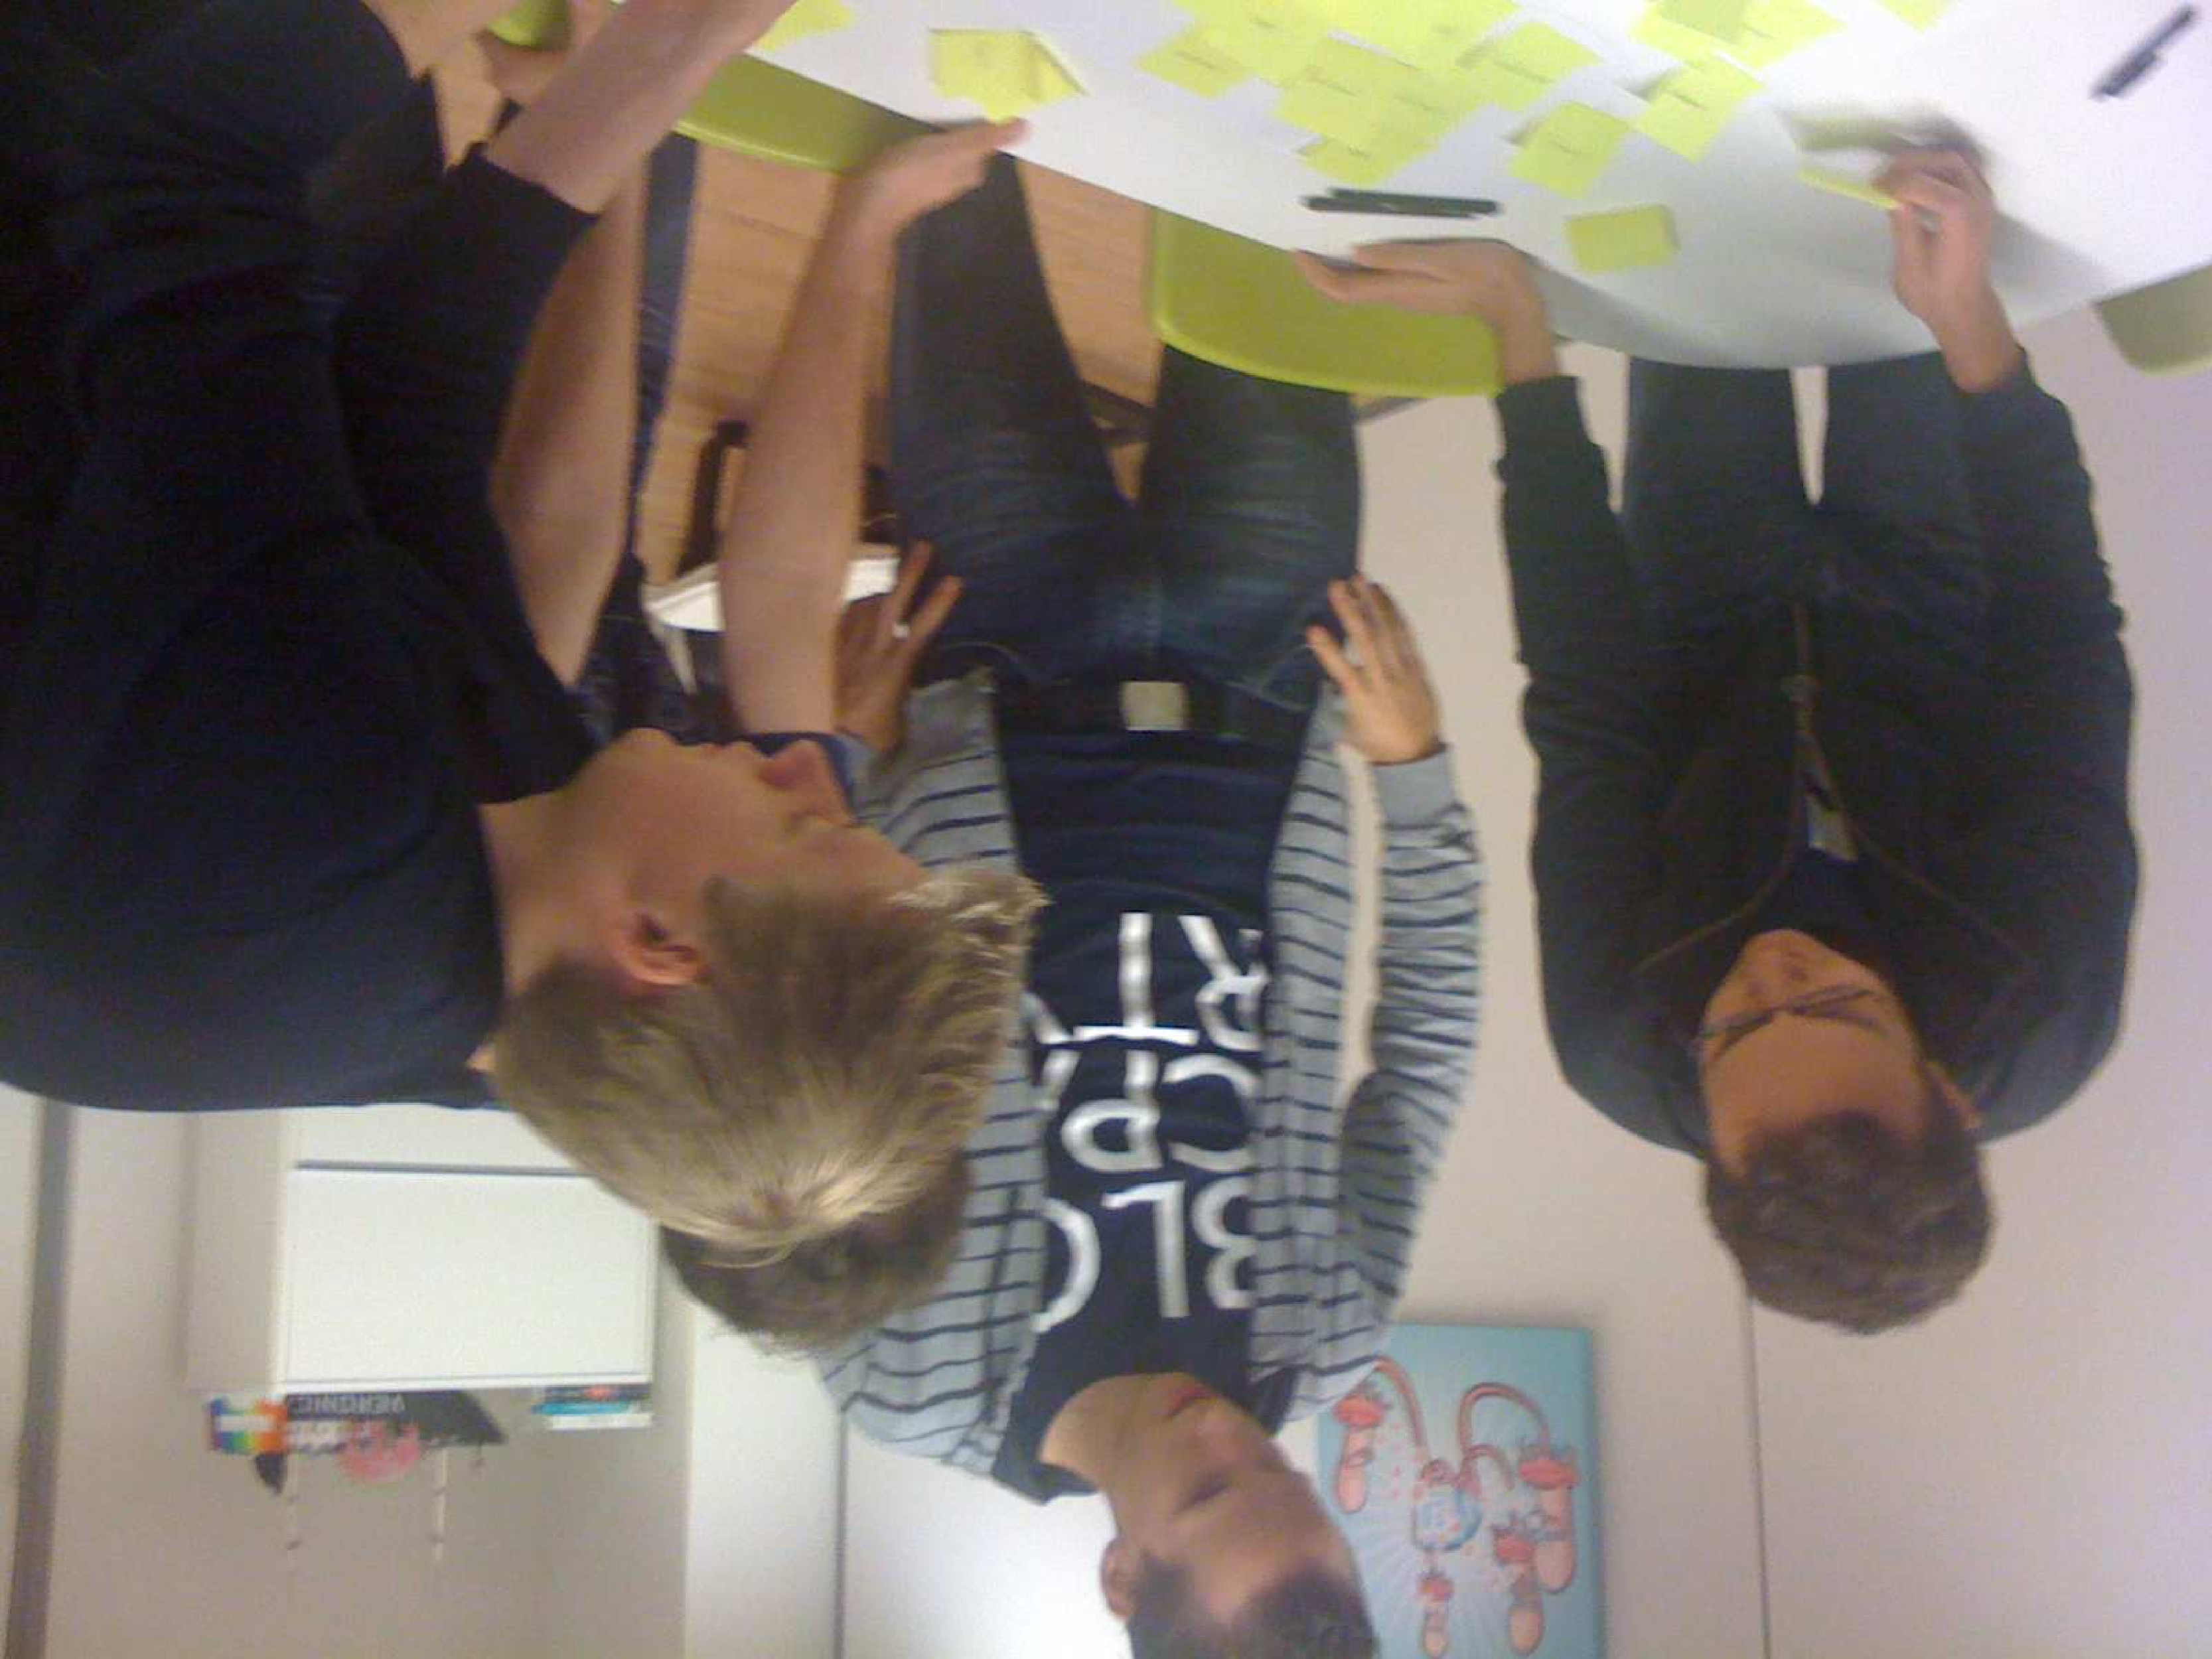
\includegraphics[height=4.5cm,angle=180]{../images/navigatie-workshop/workshopimg2}}
        \subfigure{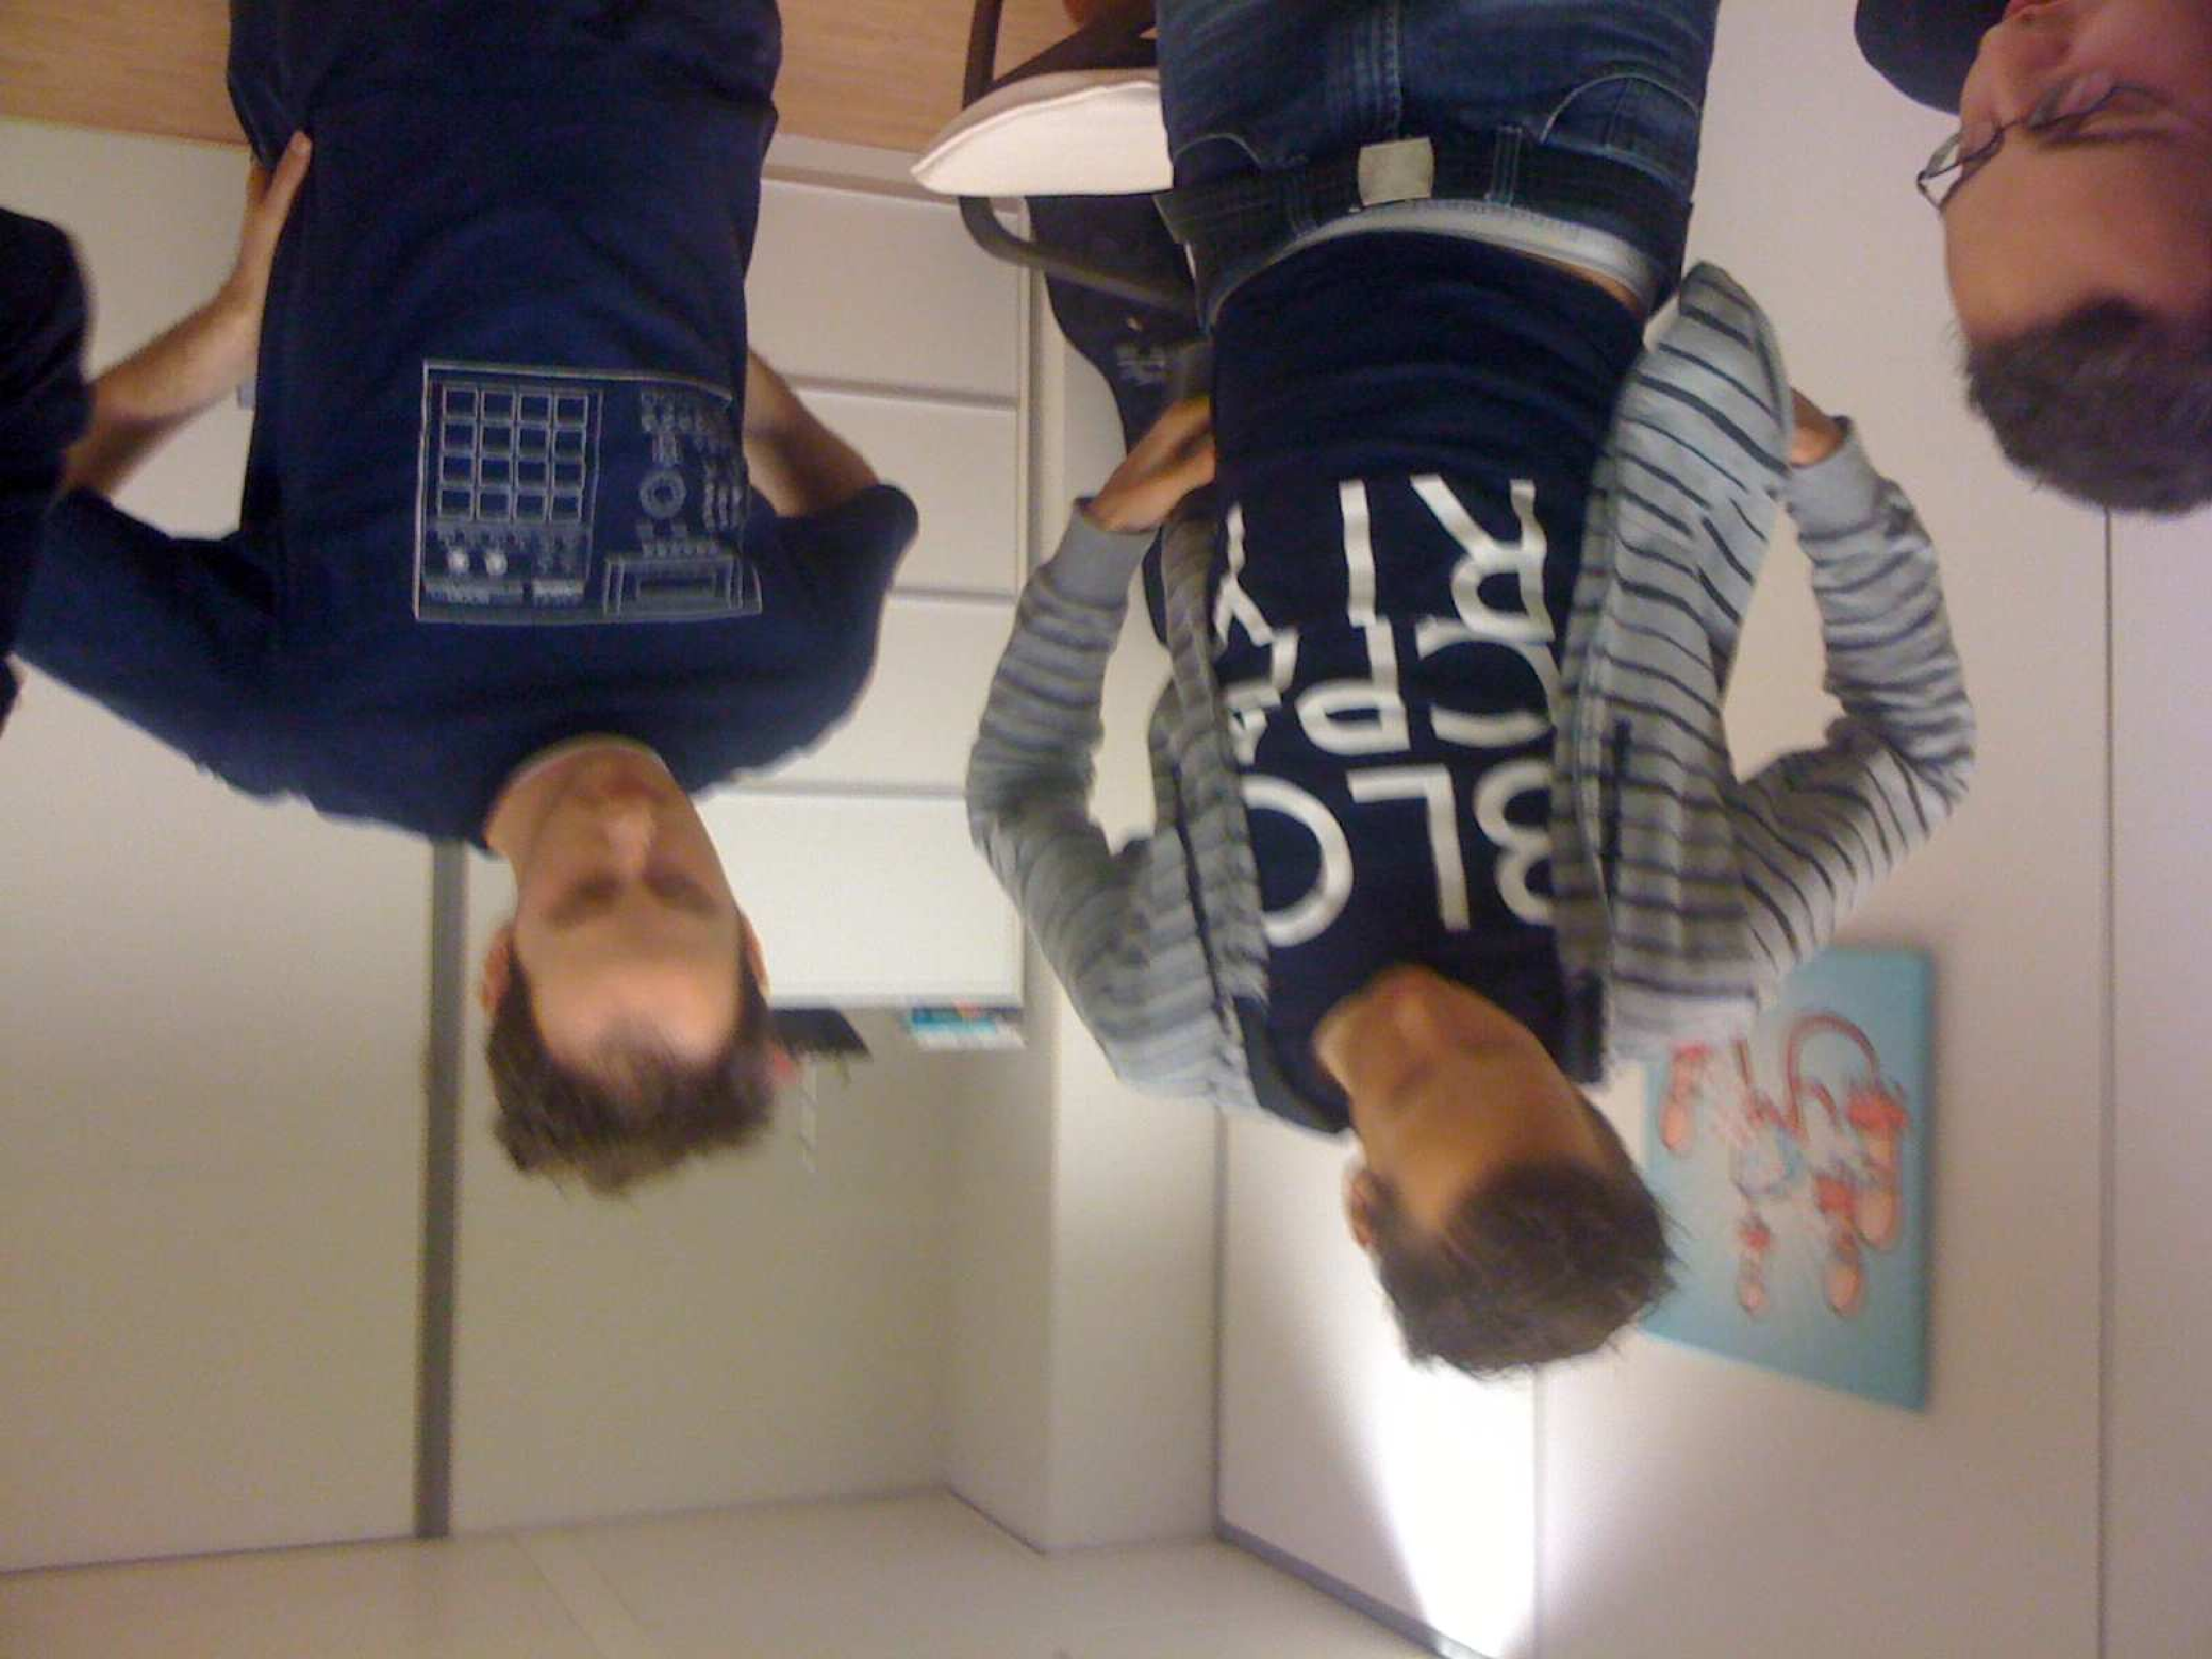
\includegraphics[height=4.5cm,angle=180]{../images/navigatie-workshop/workshopimg4}}
        \subfigure{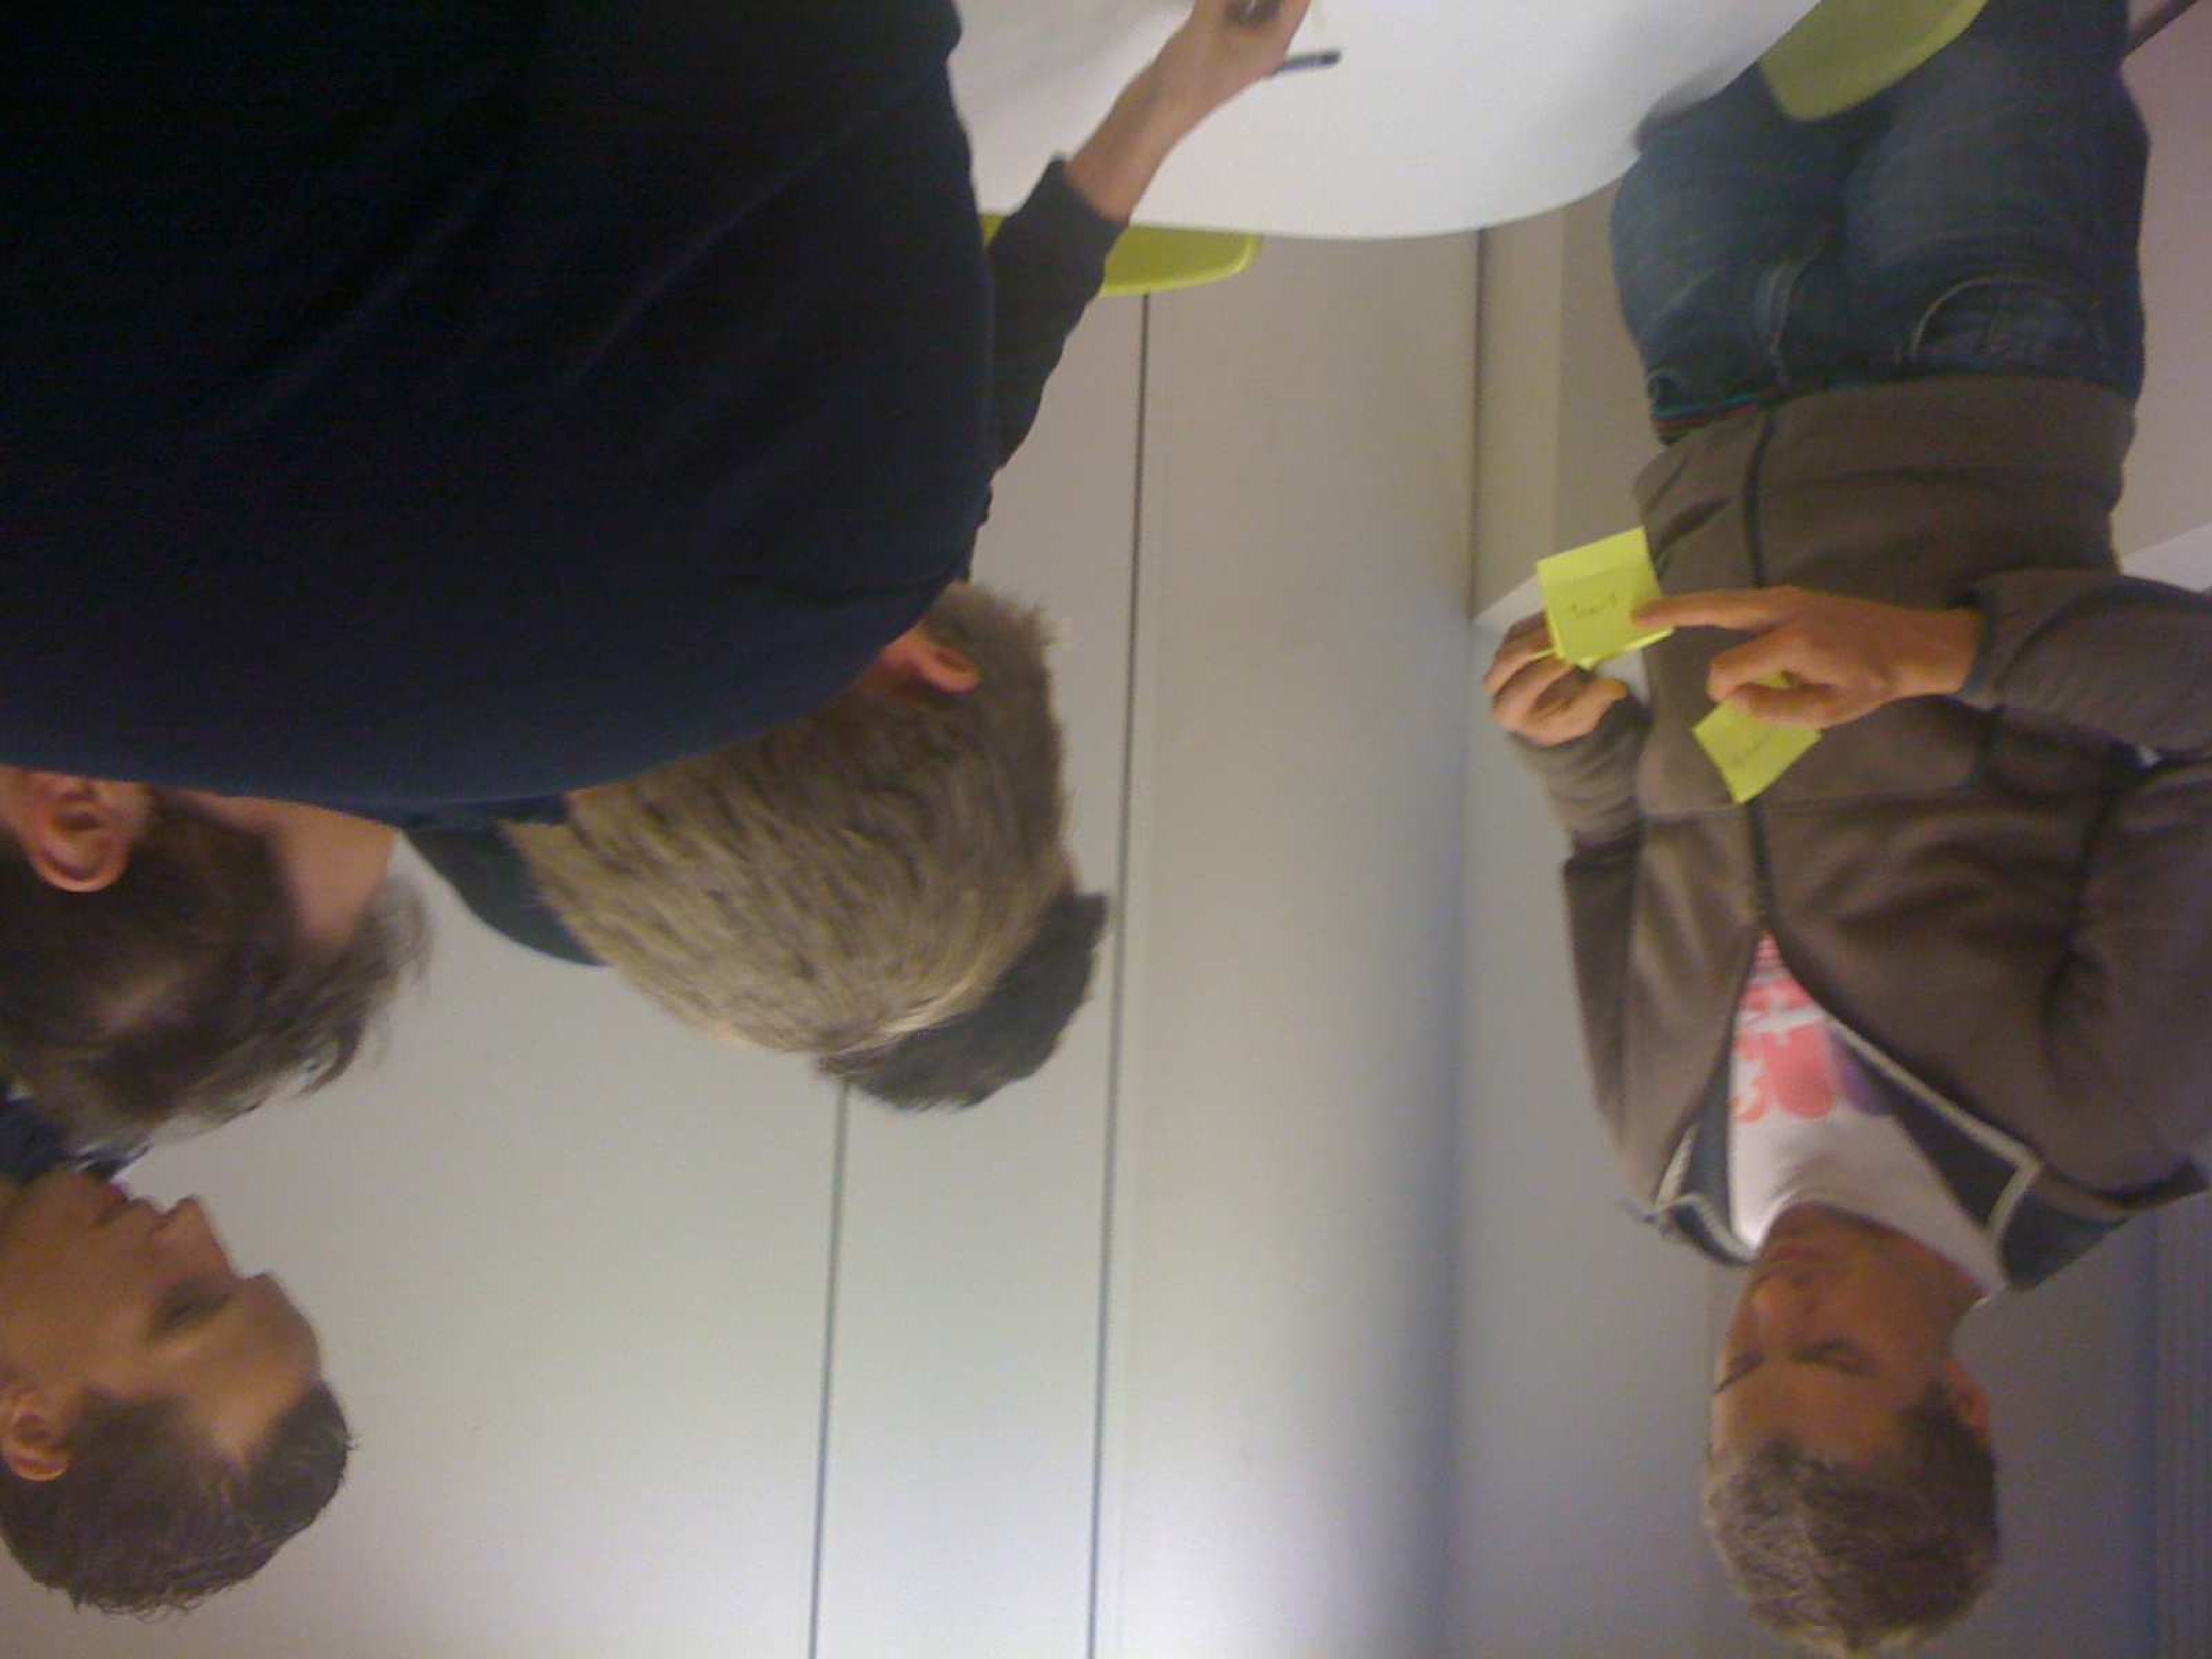
\includegraphics[height=4.5cm,angle=180]{../images/navigatie-workshop/workshopimg5}}
        \subfigure{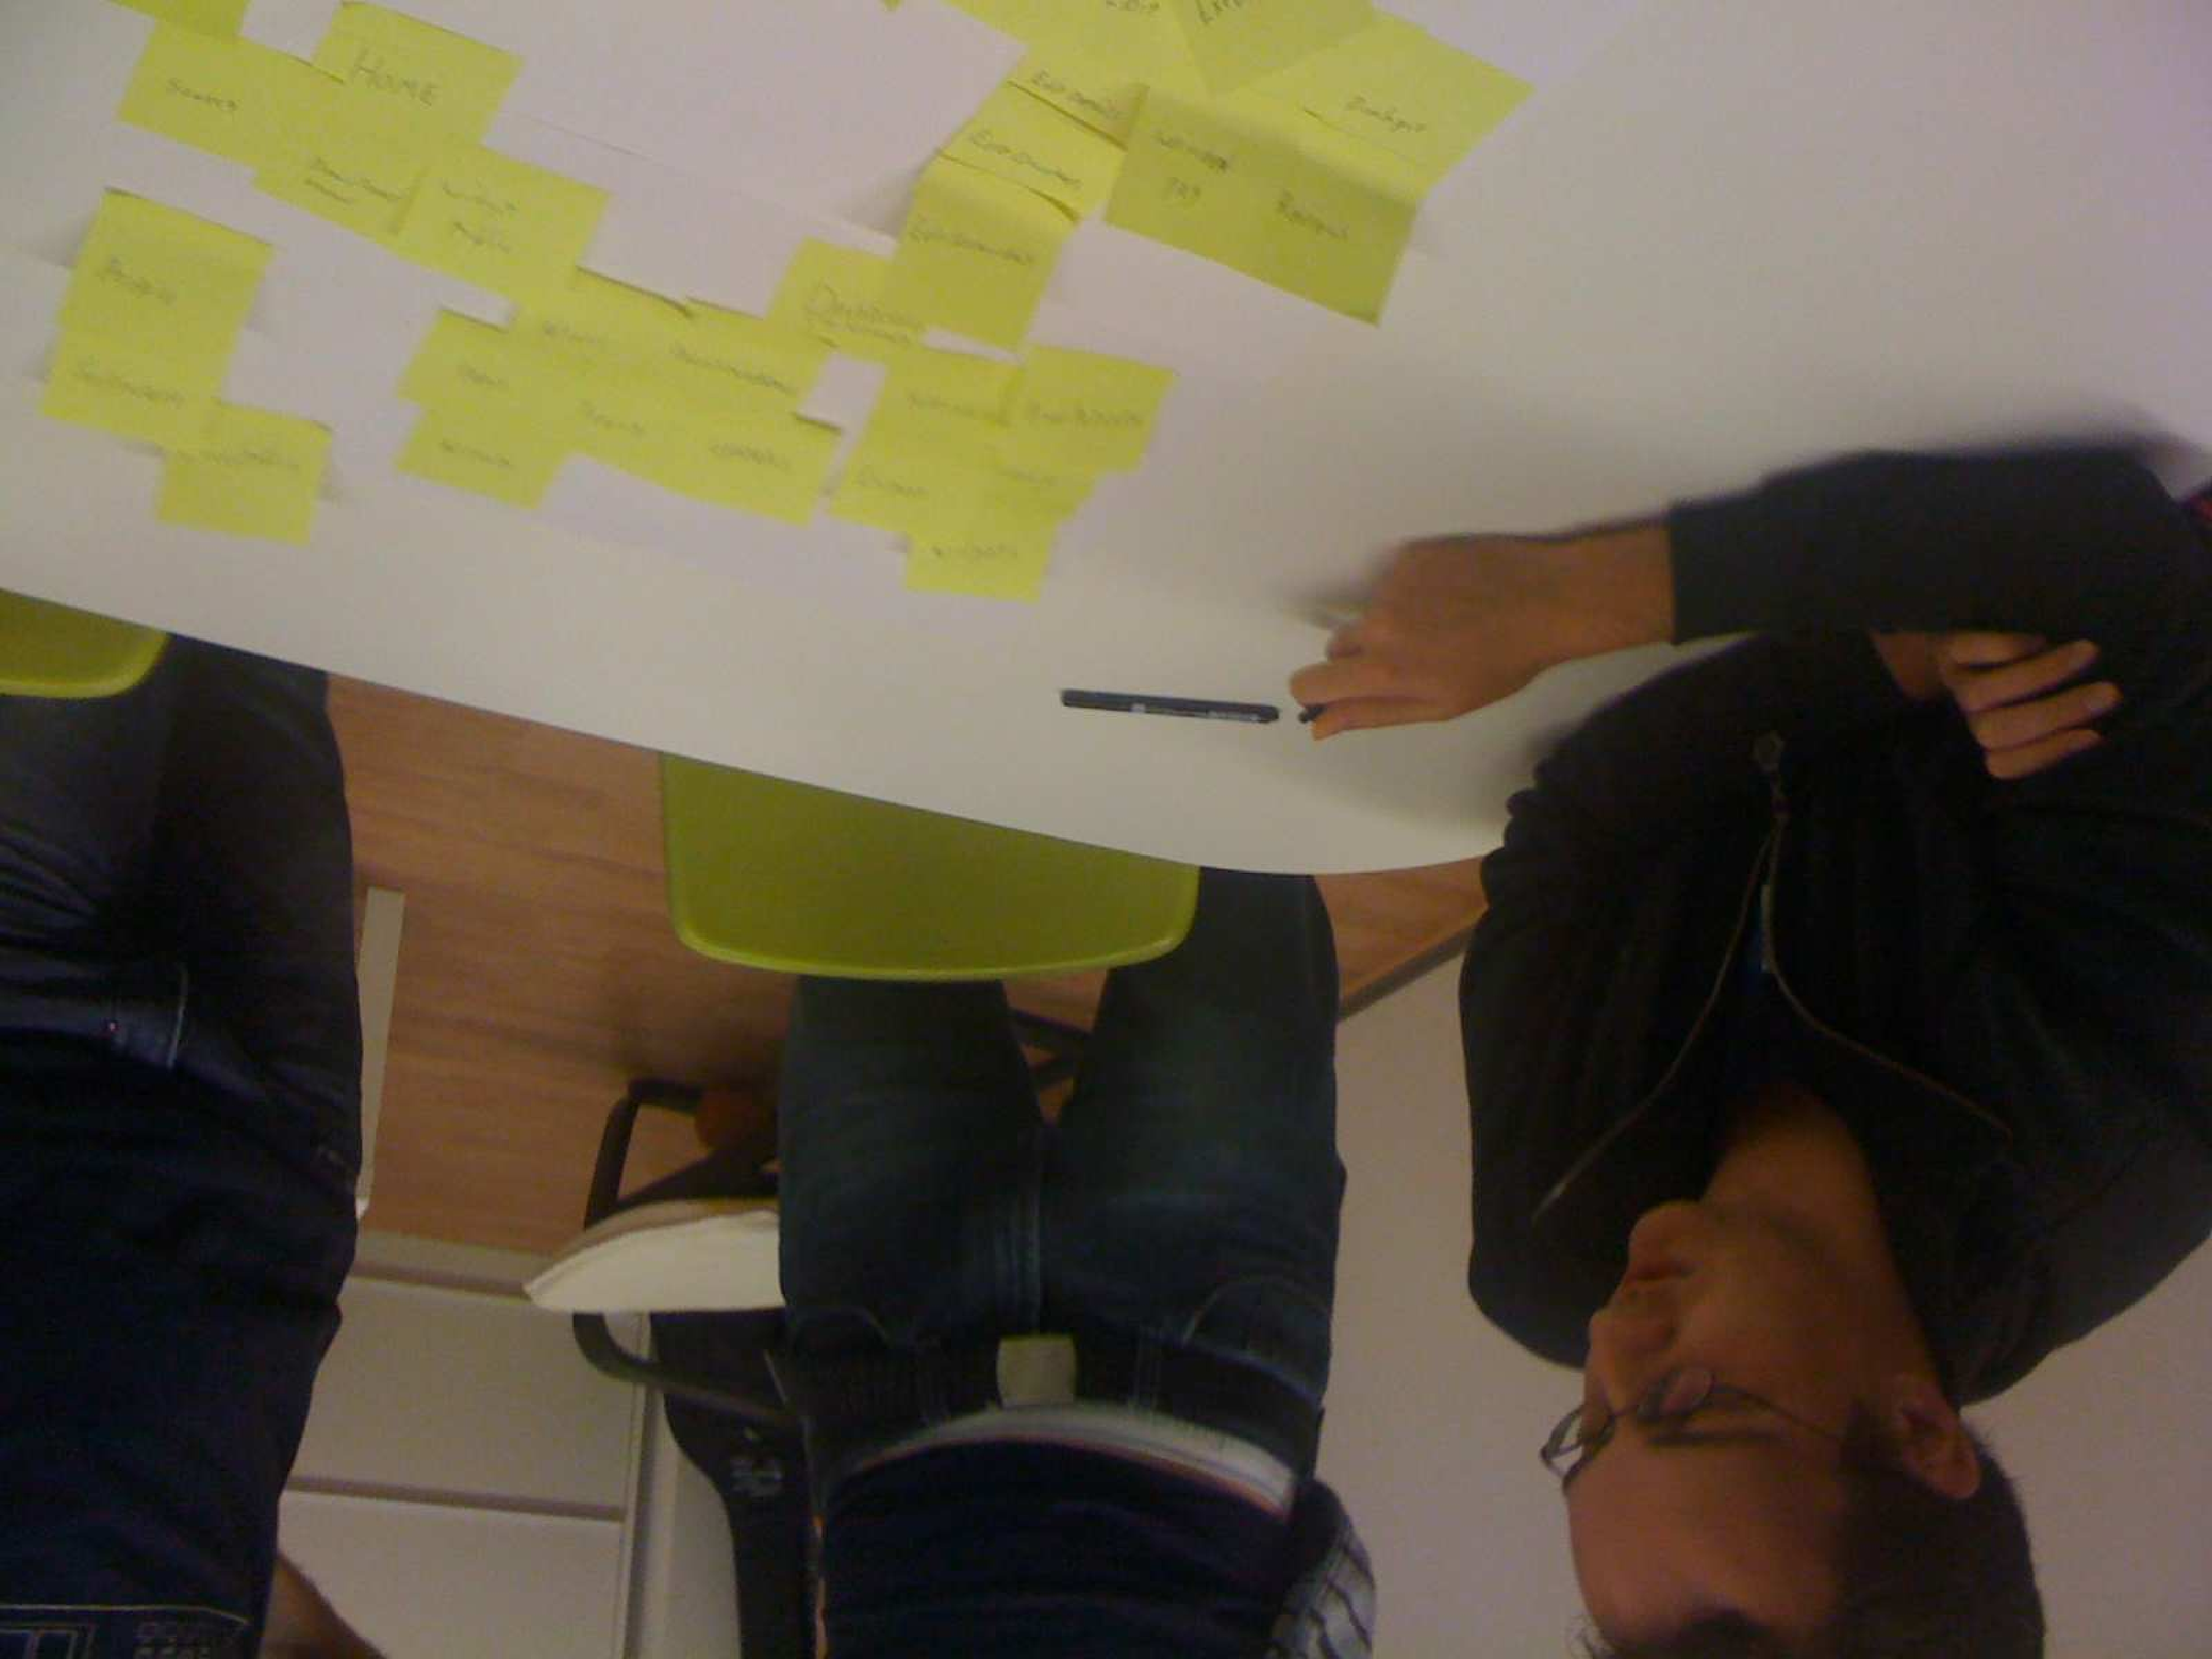
\includegraphics[height=4.5cm,angle=180]{../images/navigatie-workshop/workshopimg6}}
      \end{center}
    \end{figure}

